\documentclass{beamer}


\usepackage{amsmath,amssymb,amsfonts}
\usepackage{hyperref}
\usepackage[english]{babel}
\usepackage{times}
\usepackage[T1]{fontenc}

\mode<presentation>

  \usetheme{Warsaw}
  

  \setbeamercovered{transparent}

\def\R{{\mathbb R}}
\def\C{{\mathbb C}}
\def\bS{{\mathbb S}}

\title[] % (optional, use only with long paper titles)
{Blocked Gibbs Sampler\\ for RNA Secondary Structure Prediction from Unaligned Sequences}

\subtitle {\em Chip's Lab Meeting\\} % (optional)

\author[] % (optional, use only with lots of authors)
{Donglai Wei and Charles Lawrence$^1$}

\institute[ ] % (optional, but mostly needed)
{$^1$Division of Applied Mathematics,Brown University}

\date[ ] % (optional)
{Nov.10 2001}

\subject{Talks}
% This is only inserted into the PDF information catalog. Can be left
% out.



% If you have a file called "university-logo-filename.xxx", where xxx
% is a graphic format that can be processed by latex or pdflatex,
% resp., then you can add a logo as follows:

\pgfdeclareimage[height=1.5cm]{dna}{dna.jpg}
\logo{\pgfuseimage{dna}}



% Delete this, if you do not want the table of contents to pop up at
% the beginning of each subsection:
%\AtBeginSubsection[]
%{
%  \begin{frame}<beamer>
%    \frametitle{Outline}
%    \tableofcontents[currentsection,currentsubsection]
%  \end{frame}
%}


% If you wish to uncover everything in a step-wise fashion, uncomment
% the following command:

%\beamerdefaultoverlayspecification{<+->}


\begin{document}
\section{Title}
\begin{frame}
  \titlepage
\end{frame}

\section{Roadmap}
\begin{frame}
{\bf Roadmap} 
\textbf{1.} Background: RNA alignment and structure prediction\\
\vspace{0.5cm}
\textbf{2.} Algorithm: Blocked Gibbs Sampling \\
\vspace{0.5cm}
\textbf{3.} Results
\vspace{0.5cm}
\end{frame}

\section{Background}{\bf Background: the Prediction Problem}\\
\vspace{1.0cm}
\textbf{1.} RNA alignment(A) prediction\\
\vspace{0.5cm}
\textbf{2.} RNA consensus structure(S) prediction\\
\vspace{0.5cm}
\textbf{3.} A+S
\newpage
{\bf 1) RNA alignment(A) prediction: P(A|S)}\\
\vspace{1.0cm}
a) No S included: profile HMM \\
\vspace{0.5cm}
b) Align individual S: RNAshape \\
\vspace{0.5cm}
c) Find and assemble stems: comRNA \\
\vspace{0.5cm}
d) SCFG grammmar: CM 
\newpage
{\bf 2) RNA consensus structure(S) prediction: P(S|A)}\\
\vspace{1.0cm}
a) Individual Structure+Mutal Information: RNAlifold \\
\vspace{0.5cm}
b) Maximum weighted Matching: MWM \\
\newpage
{\bf 3) A+S: P(A,S)}\\
\vspace{1.0cm}
a) Dynamic Programming: Sankoff et.al\\
\vspace{0.5cm}
b) Iterate between A and S: \\
\vspace{0.5cm}
    i) RNAsampler(stem) \\
    ii) MASTR(MCMC local change)

\newpage
\section{Algorithm}{\bf  Probablistic Model}\\
\vspace{0.5cm}
$P(\vec A,\vec S|\Lambda_{A},\Lambda_{S},\vec Q)$ \\
\vspace{0.2cm}
{\bf Observation:}\\
\vspace{0.1cm}
$\vec Q$: Sequences\\
\vspace{0.2cm}
{\bf Hidden Variables:}\\
\vspace{0.1cm}
$\vec A$: Alignment\\
\vspace{0.1cm}
$\vec S$: Consensus Structure\\
\vspace{0.2cm}
{\bf Prior:}\\
\vspace{0.1cm}
$\Lambda_{\vec A}$: Prior for Alignment model\\
\vspace{0.1cm}
$\Lambda_{\vec S}$: Prior for Structure model\\
\vspace{0.1cm}
\newpage
{\bf Visualization:}\\
\begin{picture}(200,180)(0,0) 
\put(0,0){\resizebox{9 cm}{!}{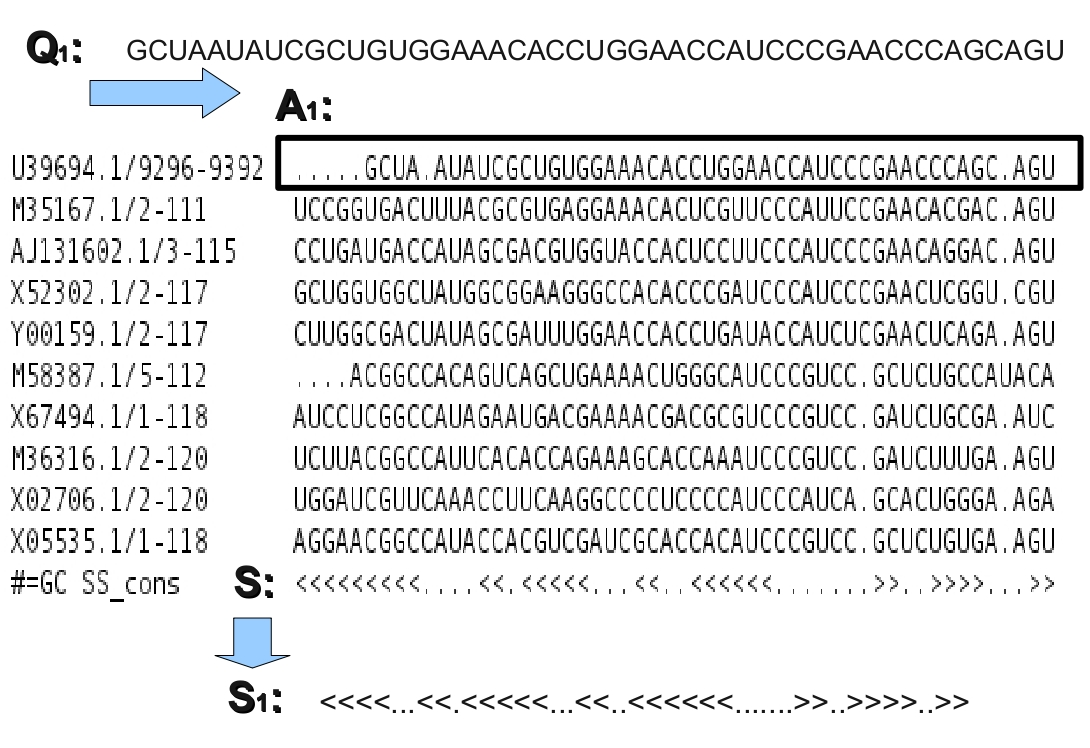
\includegraphics{si.jpg}}}
\end{picture}

\newpage
{\bf  Blocked Gibbs Sampling}\\
\vspace{1.0cm}
\textbf{1.} Initial alginment: $\vec A^{0}$\\
\vspace{0.5cm}
\textbf{2.} Iteration:\\
\vspace{0.2cm}
a) Sample $\vec S^{t+1}$ from P($\vec S^{t+1}|\vec A^{t}$)\\
\vspace{0.1cm}
b) Sample $\vec A^{t+1}$ from P($\vec A^{t+1}|\vec S^{t}$)\\
\newpage
{\bf  Cluster Analysis upon samples of S}\\
\vspace{1.0cm}
\textbf{1.} Generalized Centroid Estimator\\
\vspace{0.3cm}
\textbf{2.} Bias-Variance\\
\vspace{0.3cm}
\textbf{3.} Credibility Limit\\
\vspace{0.3cm}
\textbf{4.} Distance between centroids\\
\newpage
\section{Results}{\bf Test Cases}\\
\vspace{1.0cm}
\textbf{1.} 85 alignments from 17 RNA family (Kiryu et.al.)\\
\vspace{0.2cm}
\ \ \ \textbf{a.} PPV-SEN curve for $\gamma$-centroid\\
\vspace{0.2cm}
\ \ \ \textbf{b.} Effects of number of sequences in the alignment\\
\vspace{0.2cm}
\ \ \ \textbf{c.} Detailed look into each family\\
\vspace{0.5cm}
\textbf{2.} Riboswitch Detection\\

\newpage
{\bf 1.0) Kiryu's Data}\\
\vspace{0.7cm}
From 17 RNA famililies: tRNA,5sRNA,THI,...\\
\vspace{0.5cm}
5 Subalignments for each Family\\
\vspace{0.5cm}
10 homologous Sequences for each Subalignment\\
\begin{picture}(200,200)(0,0) 
\put(-20,0){\resizebox{10 cm}{!}{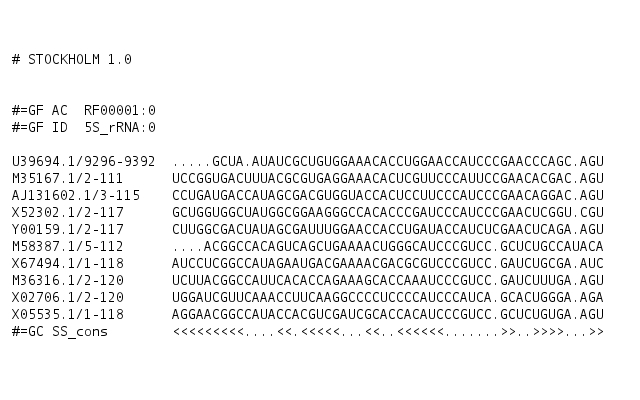
\includegraphics{data.jpg}}}
\end{picture}
\newpage
{\bf 1.1) PPV-SEN curve}\\
\begin{picture}(200,180)(0,0) 
\put(60,0){\resizebox{7 cm}{!}{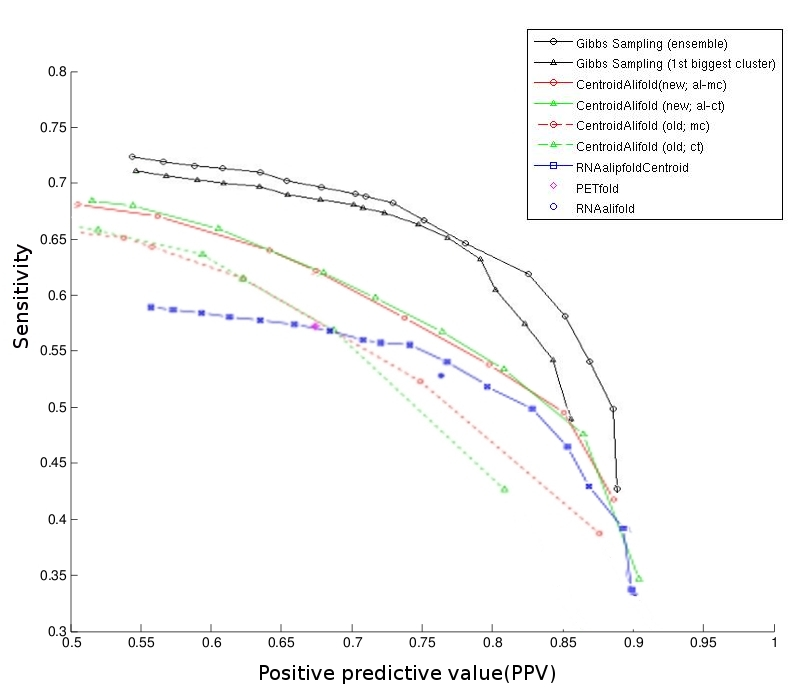
\includegraphics{haha.jpg}}}
\end{picture}
\newpage
{\bf 1.2) Varying number of Sequences in the Alignment}\\
\begin{picture}(200,170)(0,0) 
\put(-40,0){\resizebox{12 cm}{!}{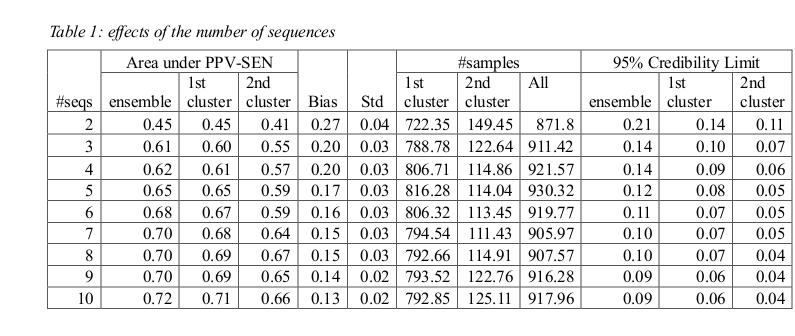
\includegraphics{table2.jpg}}}
\end{picture}
\newpage
{\bf 1.3) Look into each Family}\\
\begin{picture}(200,160)(0,0) 
\put(-20,0){\resizebox{11.5 cm}{!}{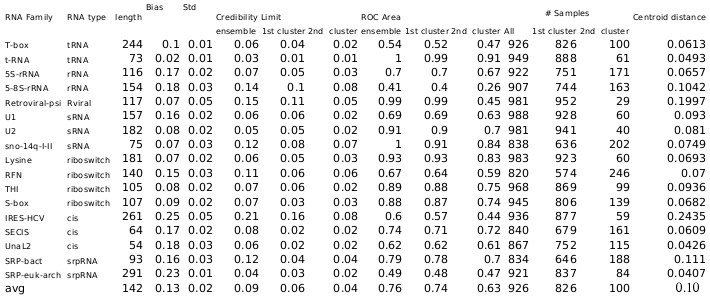
\includegraphics{new_ta.jpg}}}
\end{picture}
\newpage
{\bf 2) Side words about Riboswitch}\\
\begin{picture}(200,160)(0,0) 
\put(160,30){\resizebox{6 cm}{!}{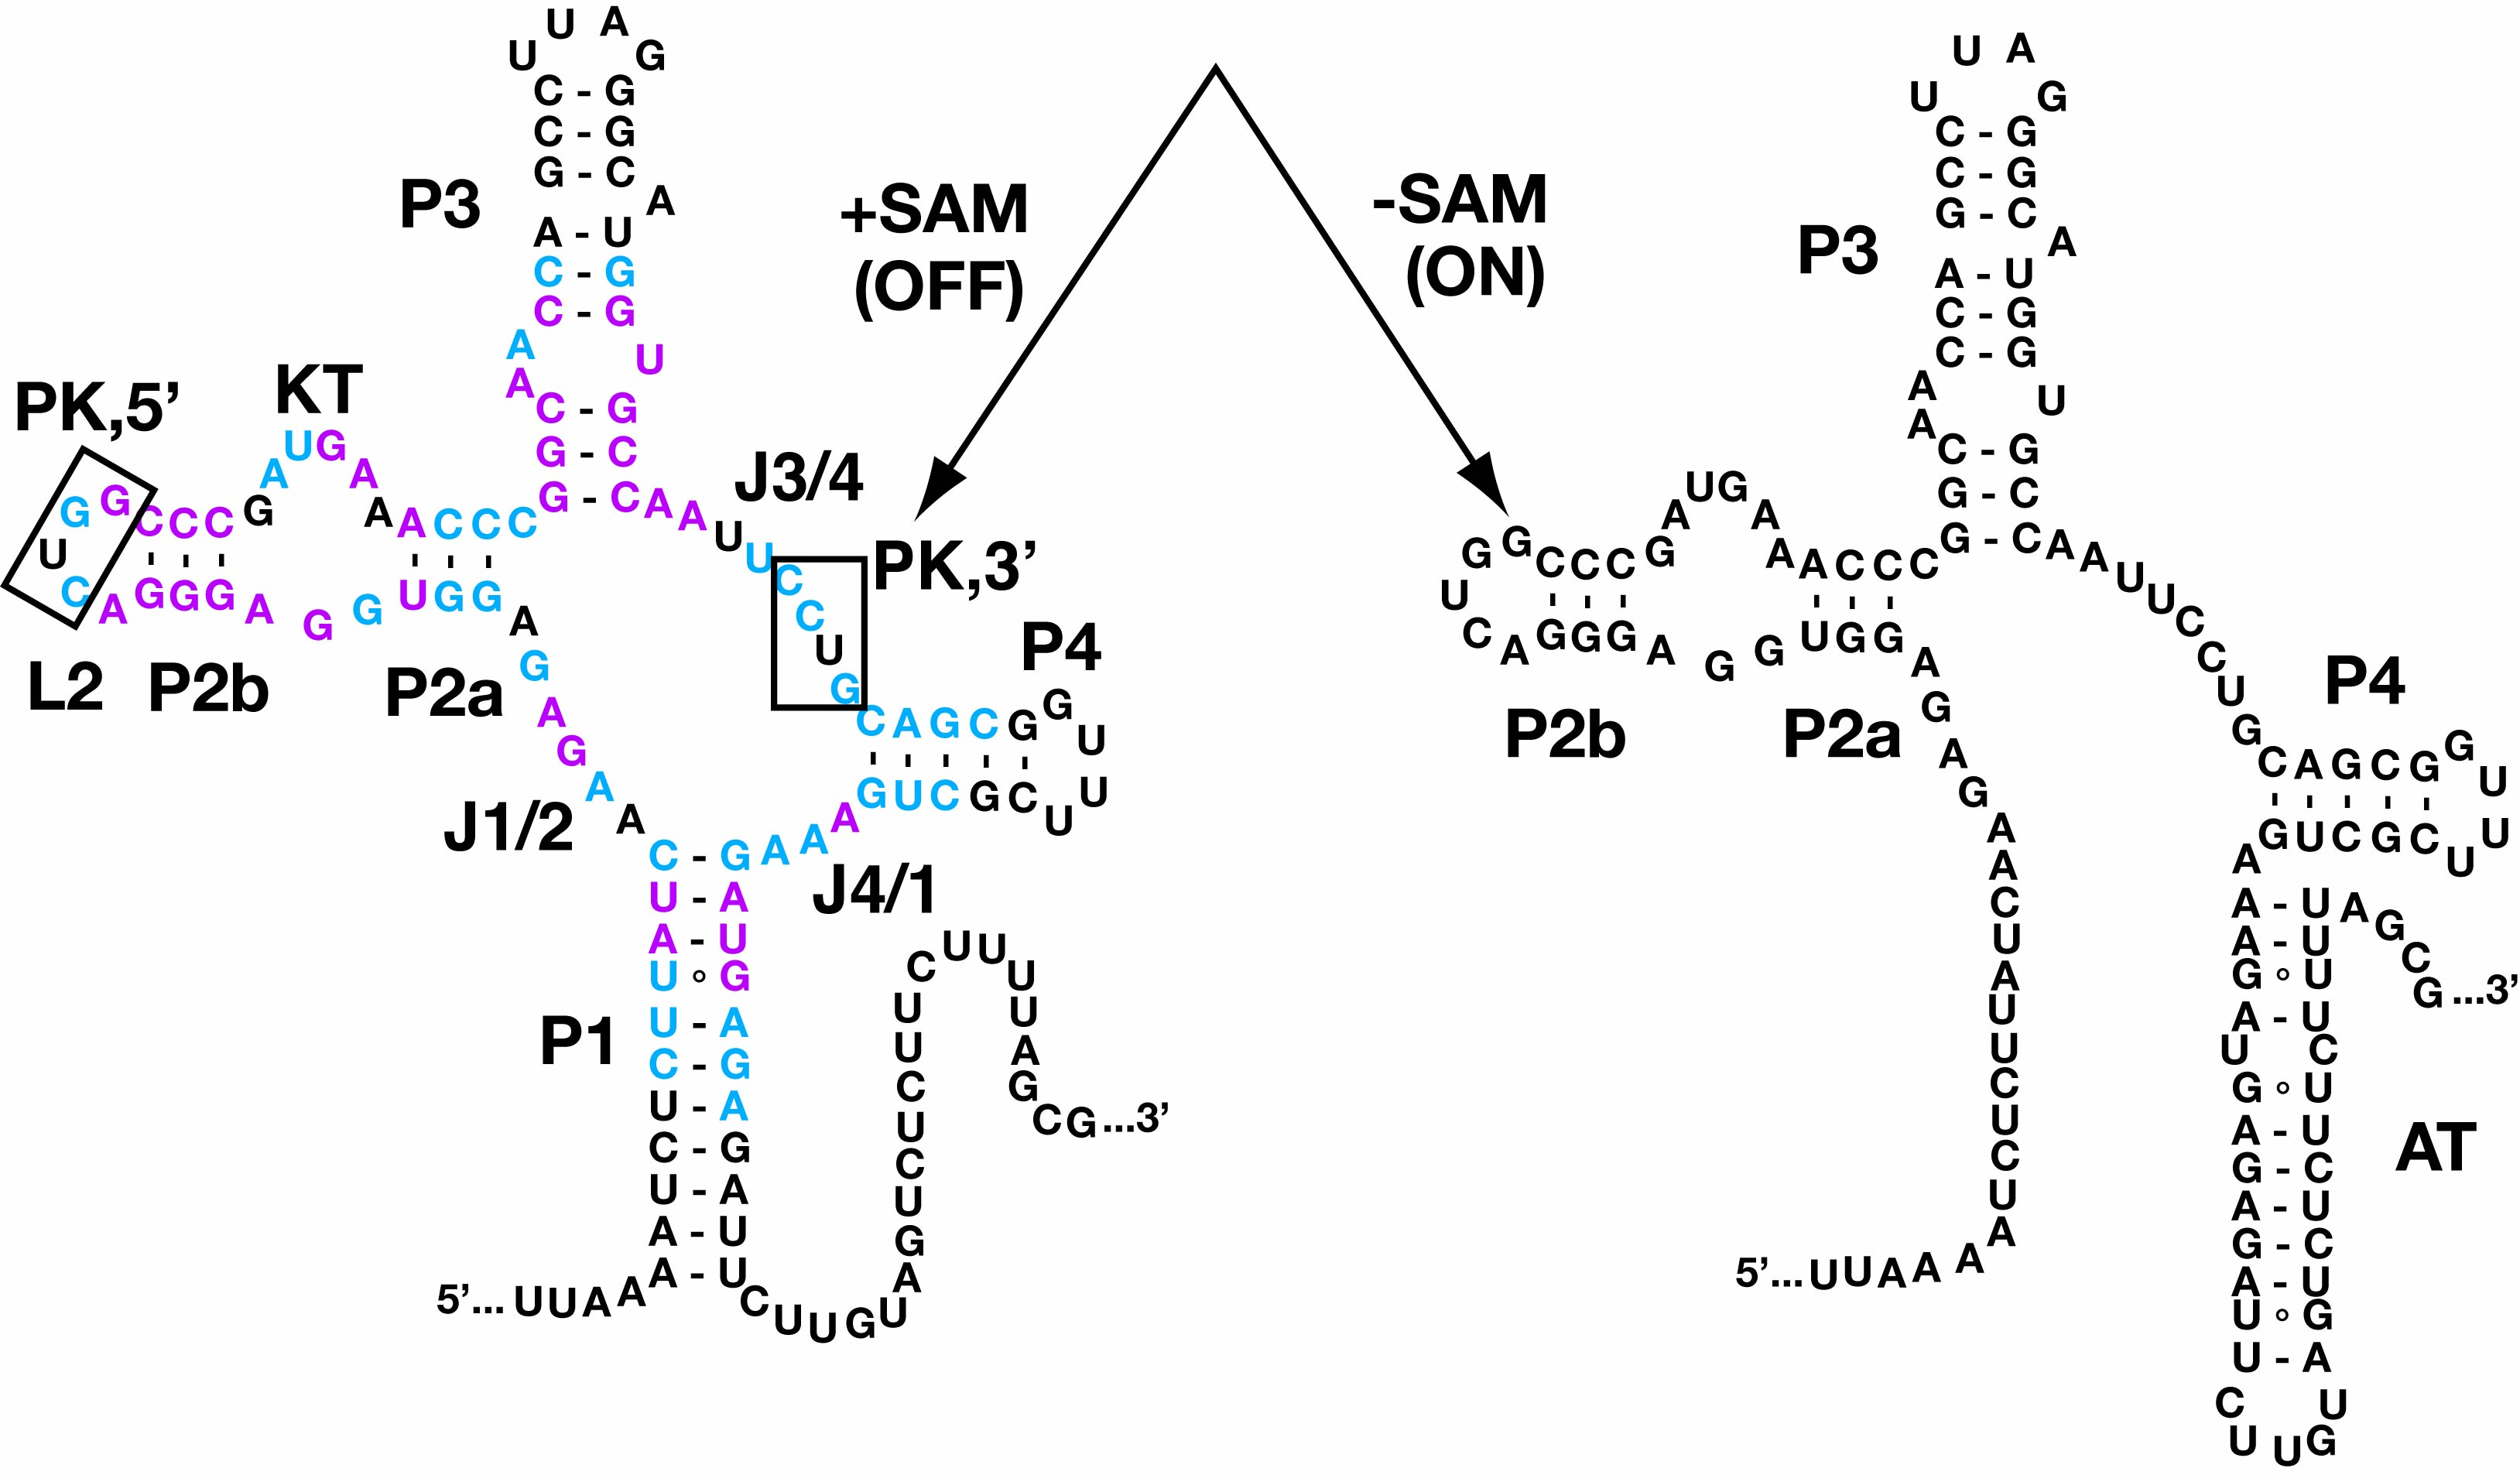
\includegraphics{ribo_g.jpg}}}
\put(-20,0){\resizebox{6 cm}{!}{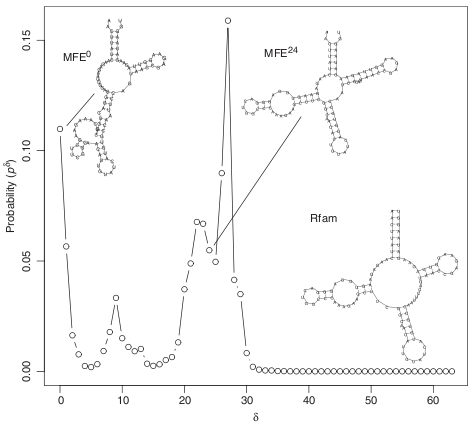
\includegraphics{ribo_n.jpg}}}
\end{picture}
\newpage
\section{Take Home Message}{\bf Take Home Message}\\
\vspace{1.0cm}
\textbf{1.} Sampling, a glimpse of the complicated probability space\\
\vspace{0.5cm}
\textbf{2.} Reference Structure, a dream never comes true\\
\newpage
\section{Acknowledgement}{\bf Acknowledgement}\\
\vspace{1.0cm}
\textbf{1.} Thanks Chip for opening the world of computation to me\\
\vspace{0.5cm}
\textbf{2.} Thanks Bill for endless technical support\\
\vspace{0.5cm}
\textbf{3.} Thanks Everyone here for enduring the torture of my presentation :p\\

%\newpage
%\section{Bibliography}{\bf Bibliography}\\
%\begin{thebibliography}{99}
%\bibitem{lewis} A. D. Lewis. The bundle of infinite jets.
%Preprint, 2006.
%{\tiny \verb+http://penelope.mast.queensu.ca/math949/pdf/infinite-jets.pdf+}
%\end{thebibliography}

\end{document}
